\section{Introdução}
\frame{
  \frametitle{Robótica}
  \begin{block}{}
    \begin{figure}[H]
      \centering
      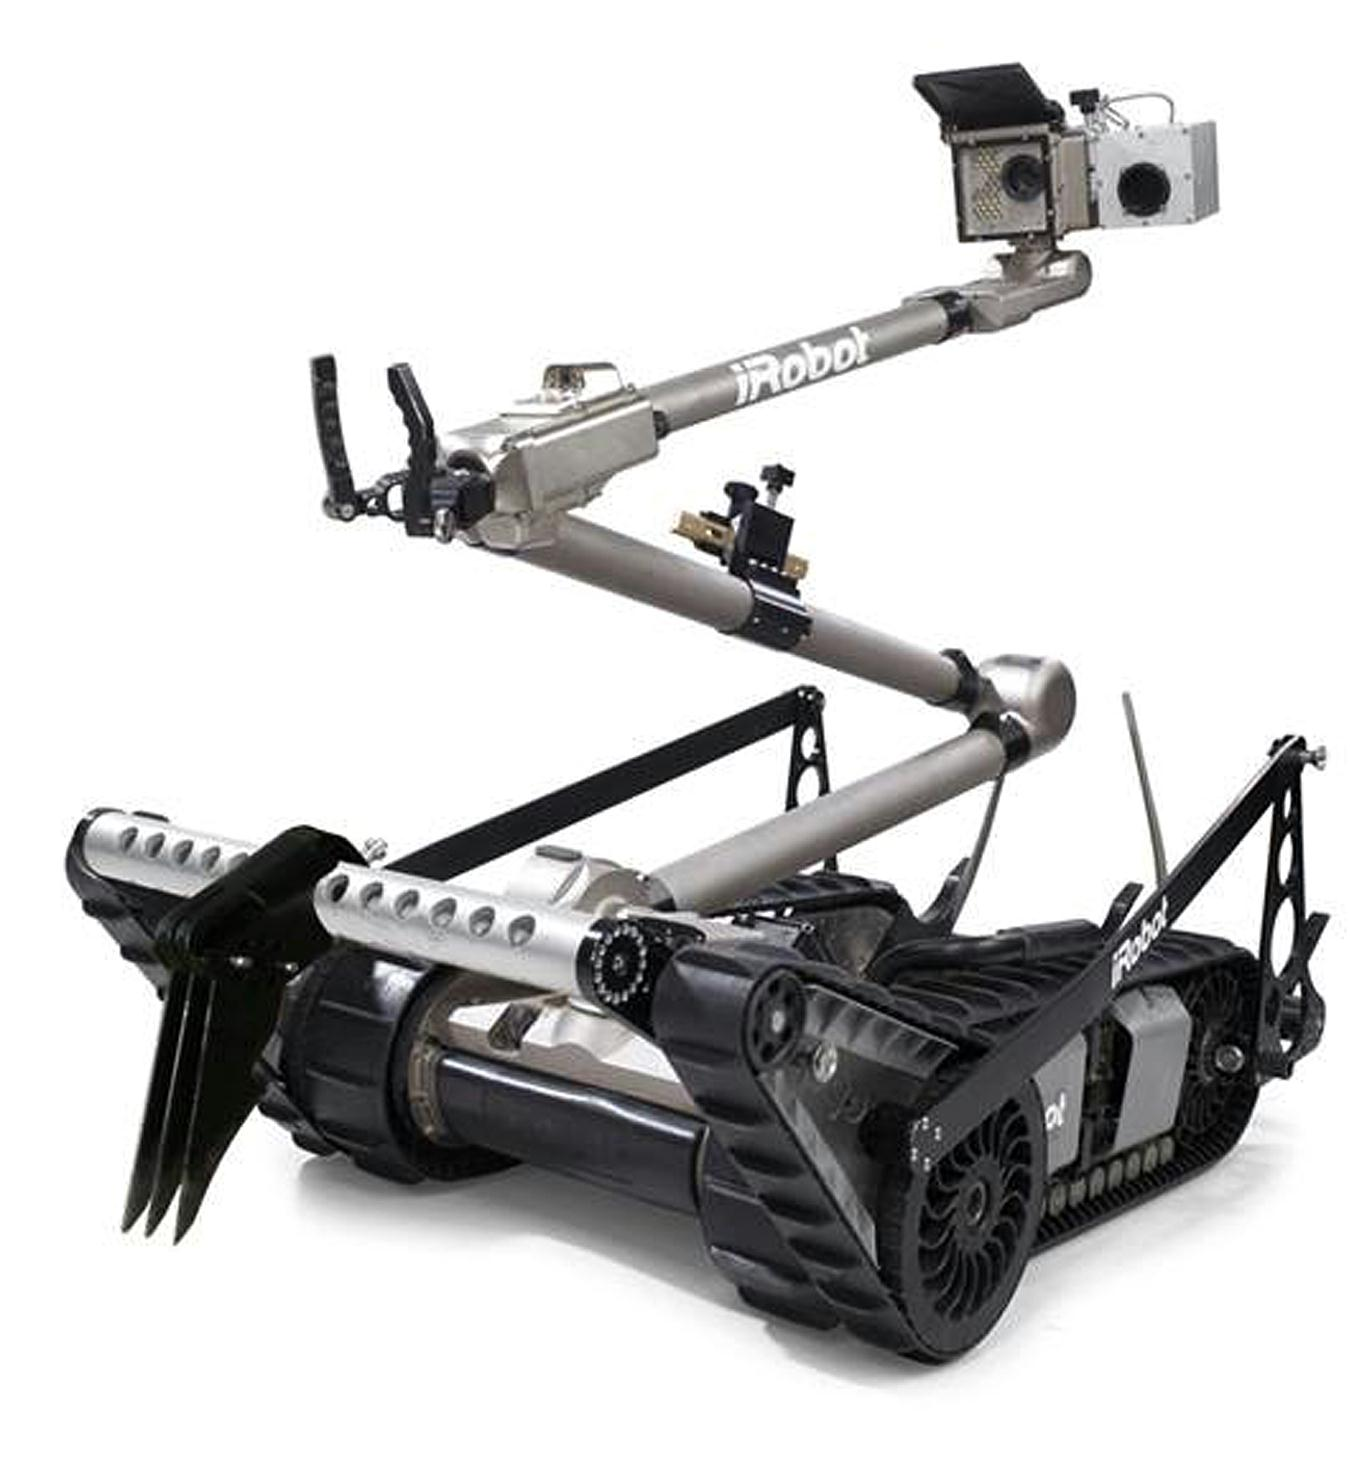
\includegraphics[width = 0.35\linewidth]
      {figuras/robotica}
       \caption{\textit{iRobot} utilizado na inspeção da
         Central Nuclear de Fukushima I após o sismo e
         tsunami de 2011 em Sendai}
    \end{figure}
  \end{block}
}
\frame{
  \frametitle{Robótica}
  \begin{block}{}
    \begin{figure}[H]
      \centering
      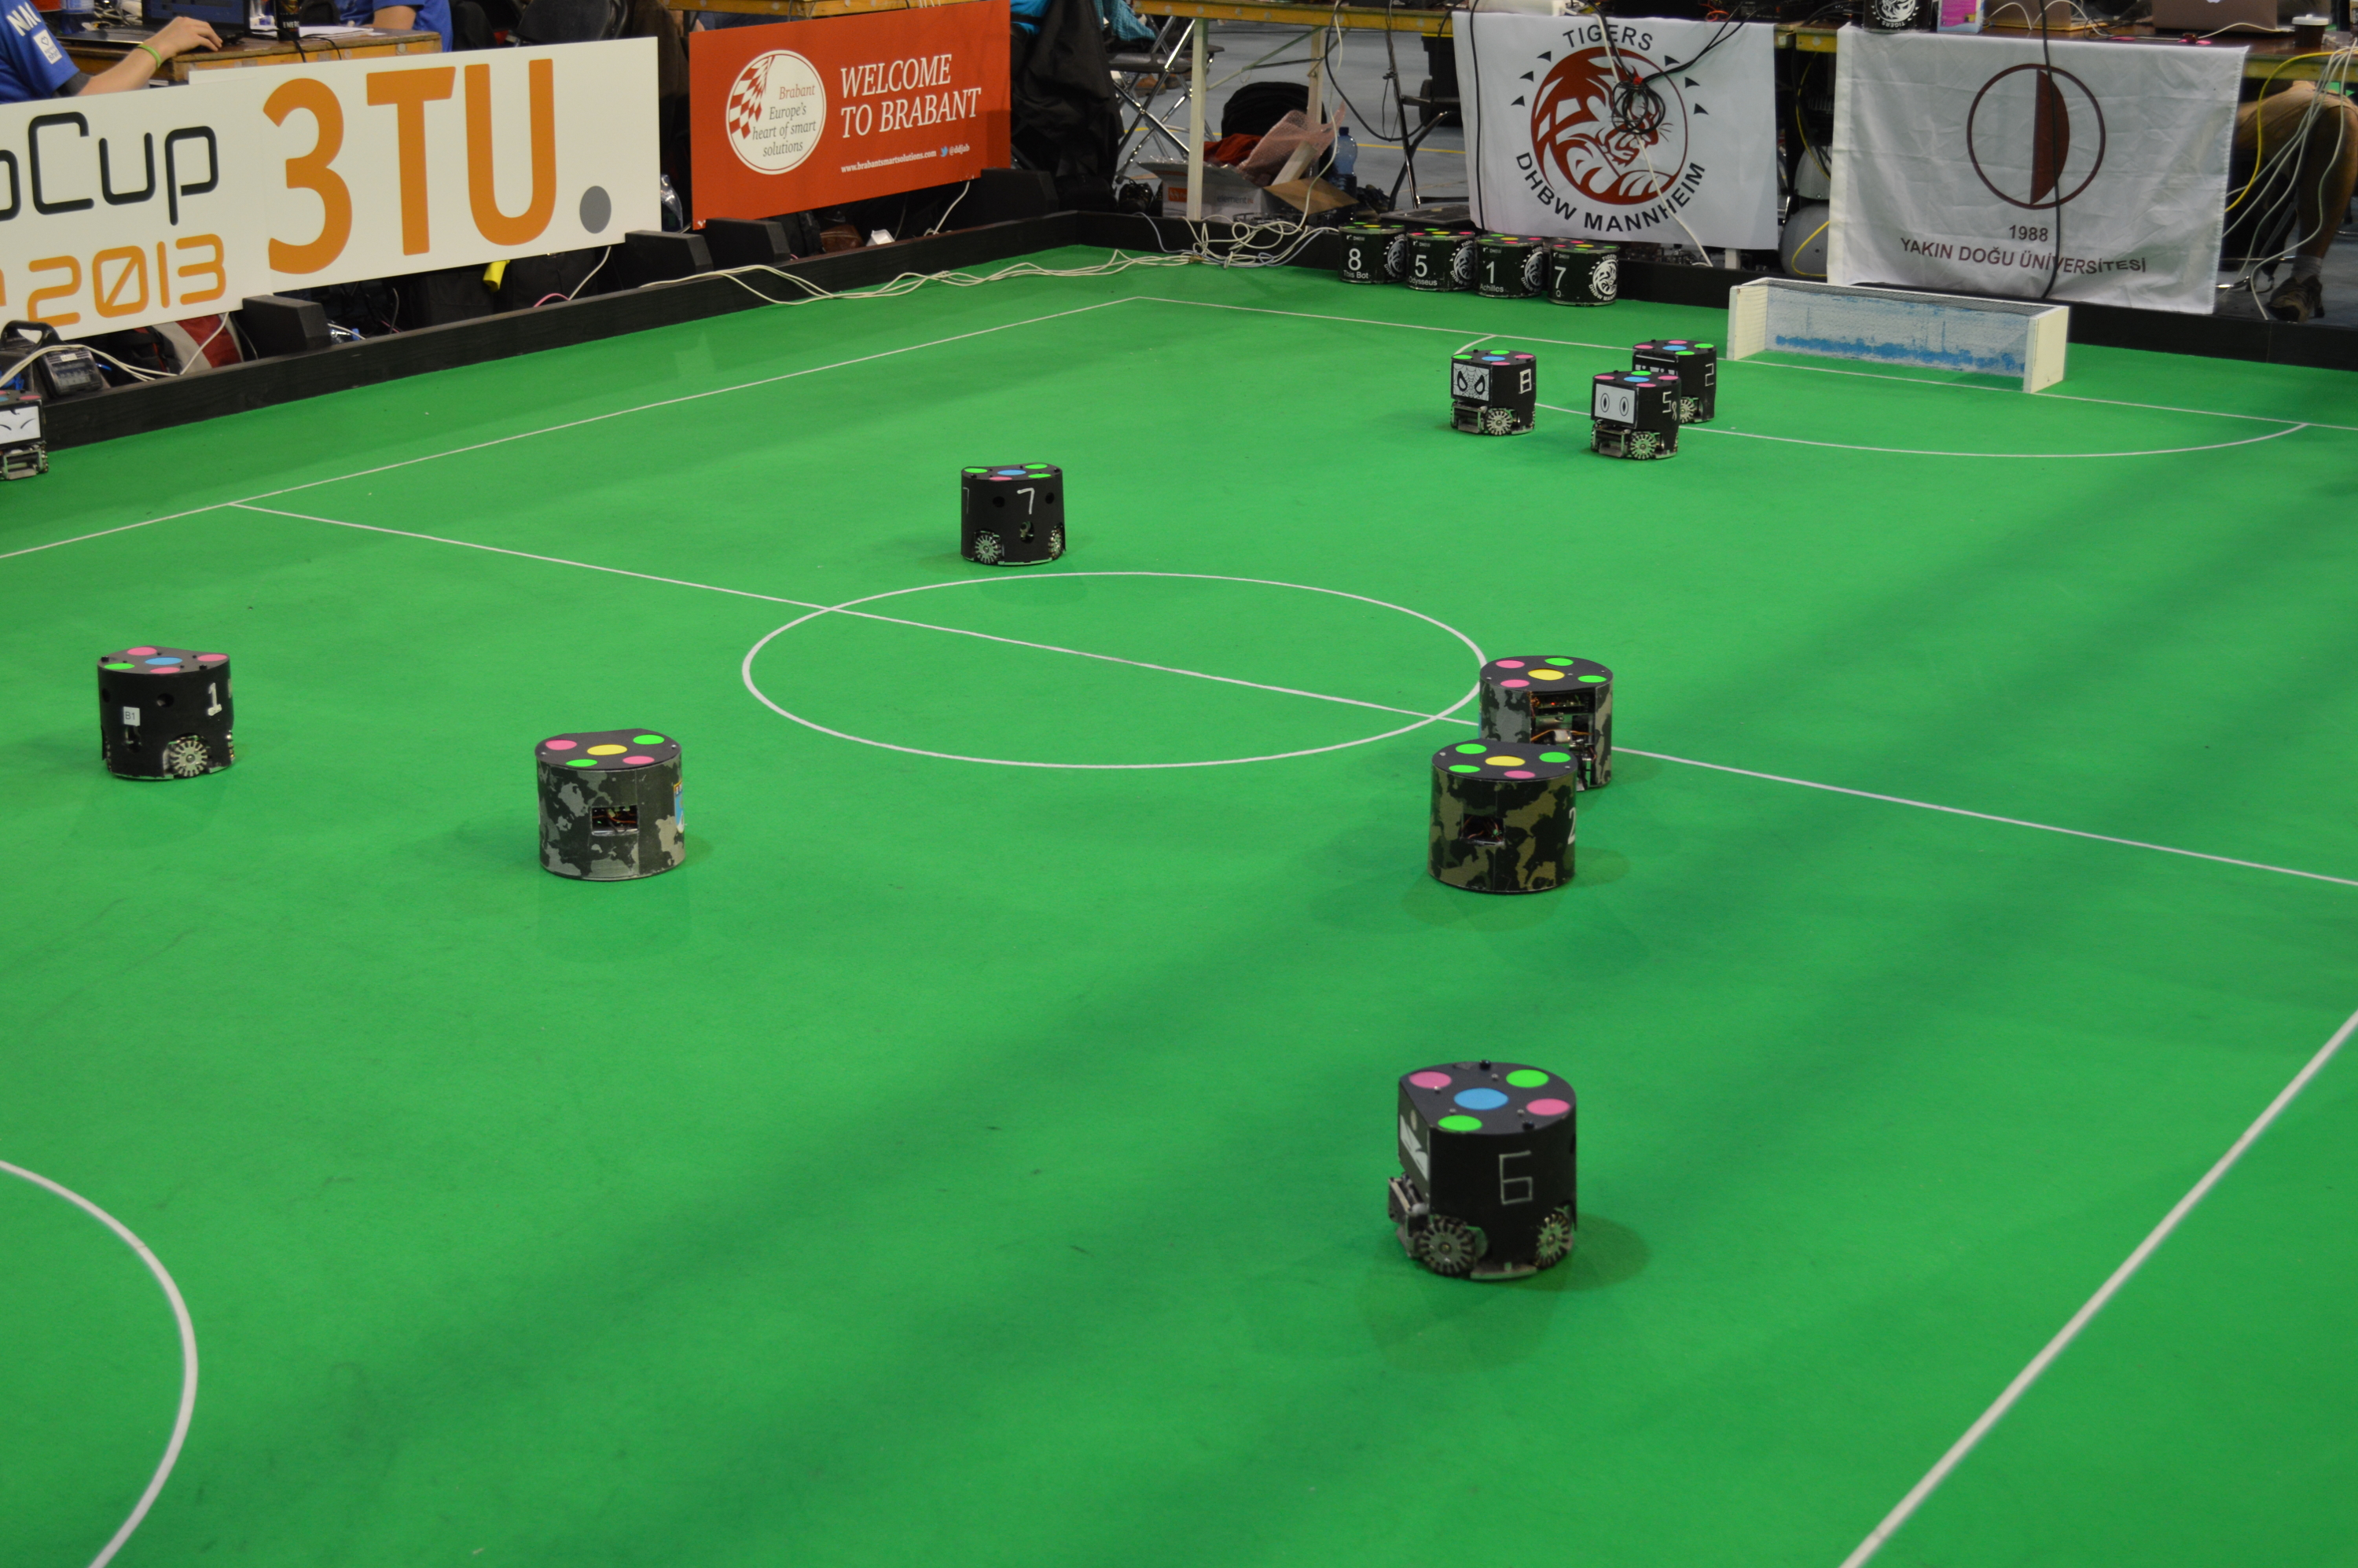
\includegraphics[width = 5cm]
      {figuras/robocup2013}
      \caption{Partida da \textit{Small Size League} (SSL)
      da Robocup 2013}
    \end{figure}
  \end{block}
}
\frame{
  \frametitle{Objetivos}
  \begin{block}{}
    \centering
    Estudar os algoritmos ACO, SA, GA, ANN e lógica fuzzy.
  \end{block}
  \begin{block}{}
    \centering
    Analisar se e como a inteligência artificial de um time de futebol de robôs
    pode ser modelada utilizando esses algoritmos e métodos com as informações
    contidas nos $logs$ (definido a seguir) de um jogo da SSL da RoboCup.
  \end{block}
}

% vim: tw=79 et sw=2 ts=2
